\chapter{Nuclear Engineering Background}
\label{cha:engineering}

\section{Advanced Gas-cooled Reactors (AGRs)} \label{AGR}

The UK nuclear power sector is dominated by the advanced gas-cooled reactor  (AGR) \cite{nonbol1996description}. There are 14 AGR reactors spread across 7 UK power stations. This design differs from most reactors around the world in that it consists of a graphite core cooled by carbon dioxide gas (as opposed to the almost ubiquitous water cooled reactor). The international novelty of this design means that all safety analysis has to be performed domestically, leading to a significant requirement for computation.

\begin{figure}[ht!]
	\centering
	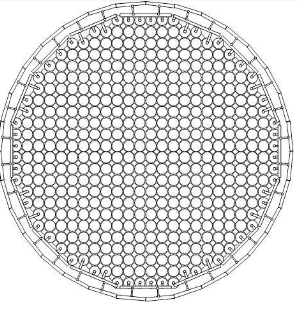
\includegraphics[scale=0.75]{Figures/AGR_plan.png}
	\caption{AGR Core Plan View}
	\label{fig:schematic}
\end{figure}

\noindent
The AGR consists of several thousand stacked graphite bricks assembled in an interlocking 3-dimensional assembly (shown in Figure~\ref{fig:schematic} and \ref{fig:side}). There are two principal brick types shown in Figure~\ref{fig:bricks}: (1) large bore bricks for the insertion of fuel assemblies and (2) interstitial bricks which provide structural support, some of which have a small bore to allow the insertion of a control rod. The bricks are linked and held in position by rectangular graphite keys. An individual stack of bricks the height of the core is known as a channel, with types of channel dictated by the type of brick i.e. fuel channels and interstitial channels.

\begin{figure}[ht!]
	\centering
	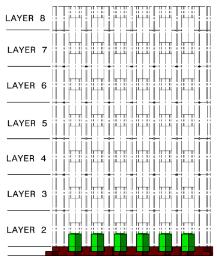
\includegraphics[scale=0.75]{Figures/AGR_side}
	\caption{AGR Core Side View}
	\label{fig:side}
\end{figure}

\noindent
The primary safety concern with the AGR is the cracking of the fuel bricks. Given enough cracks, the ability to insert fuel or control rods could be impeded. The mechanism by which the cracks occur is well understood. The intense heat and radiation cause a radio-catalytic reaction between the graphite and $CO_2$, which in turn causes a reduction in the mass and volume of the bricks. The reduced volume causes a stress differential, which leads to a concentration of stress and cracking at the root of the keyways (Figure \ref{fig:cracking}). \\ 

\noindent
The growth of these cracks ultimately results in the splitting of the brick into two halves (see Figure \ref{fig:cracked}). At any given time, it is difficult to ascertain which bricks are exhibiting cracks due to inaccessible nature of the core internals. Forecasting the location of cracks as a function of time is an area of ongoing research. 

\section{Traditional Engineering Safety Assessments} \label{Engineering}
The UK Office for Nuclear Regulation (ONR) stipulates that the AGR operator (EDF Energy) must demonstrate that the ability to control the reactor (i.e. insert control rods) will not be threatened under any circumstance i.e an earthquake or other serious event.\\

\begin{figure}[ht!]
	\centering
	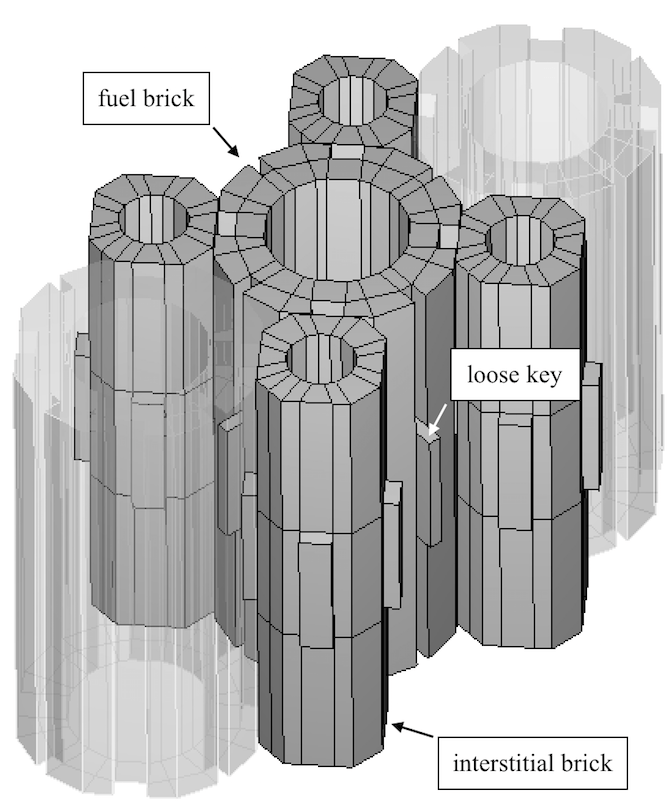
\includegraphics[scale=0.17]{Figures/brick_types_parmec}
	\caption{AGR Core Brick Types}
	\label{fig:bricks}
\end{figure}

\begin{figure}[ht!]
	\centering
	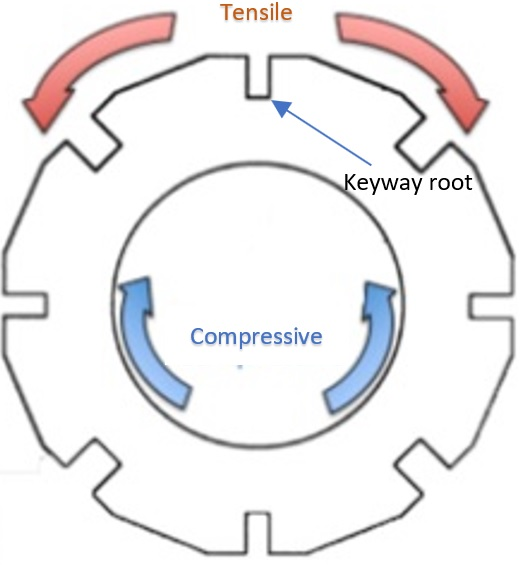
\includegraphics[scale=0.35]{Figures/cracking_mechanism}
	\caption{Brick Cracking Mechanism}
	\label{fig:cracking}
\end{figure}

\begin{figure}[ht!]
	\centering
	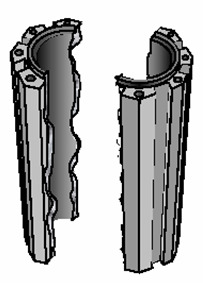
\includegraphics[scale=0.65]{Figures/Brick_Cracking}
	\caption{Cracked AGR Brick}
	\label{fig:cracked}
\end{figure}

\begin{figure}[b!]
	\centering
	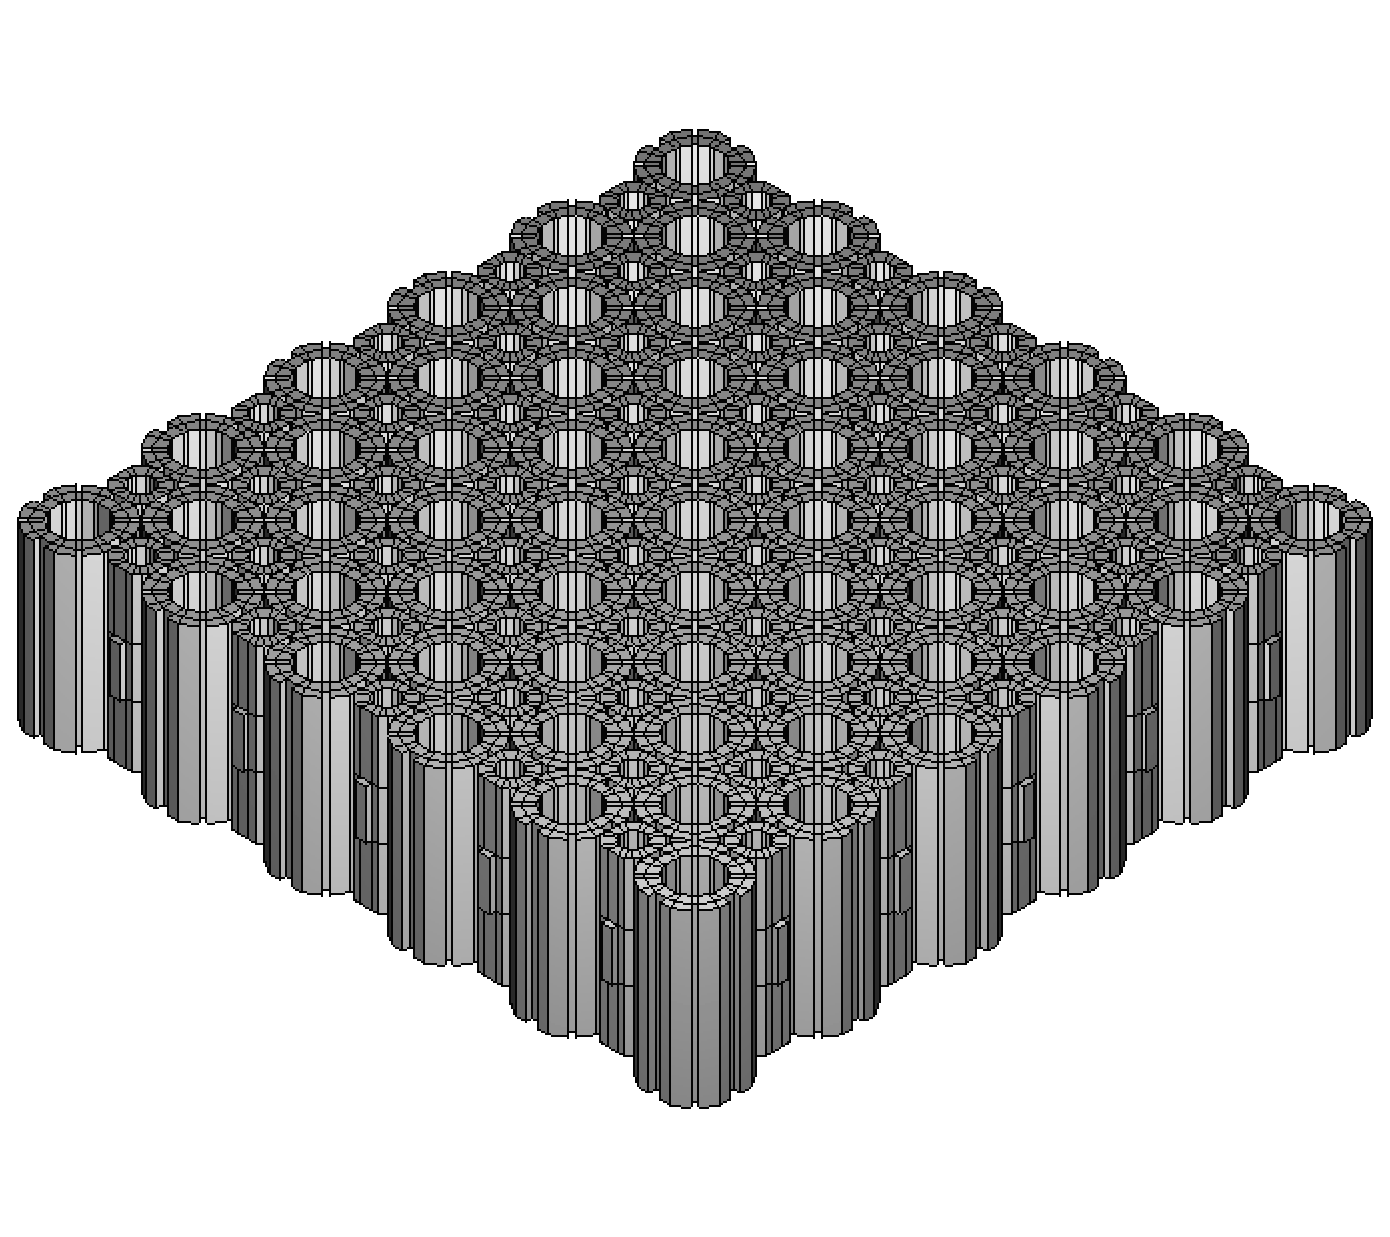
\includegraphics[scale=0.12]{Figures/parmec_bricks.png}
	\caption{Visualisation of Parmec Model}
	\label{fig:FEA}
\end{figure}

\noindent
The traditional approach used to ensure the safe condition of the AGR involves production and analysis of complex engineering models, which are deterministic and rely on physical relationships. Examples include the computational model Parmec \cite{wiki:xxx} and the physical Multi-Layer Array (MLA) model \cite{dihoru2014multi} at the University of Bristol (Figures \ref{fig:FEA} \& \ref{fig:ENG}, respectively). Both of these models are configured to to simulate a once in 10,000 year earthquake. \\

\begin{figure}[b!]
	\centering
	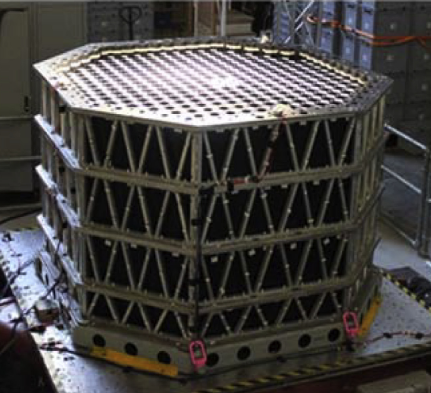
\includegraphics[scale=0.5]{Figures/MLA_rig}
	\caption{Multi-Layer Array Rig}
	\label{fig:ENG}
\end{figure}

\noindent
As mentioned at the end of section~\ref{AGR}, it is difficult to ascertain where the cracks are (or where they will occur). In lieu of actual crack positions, the traditional approach is to generate a random distribution of cracks, represented by a 3-dimensional tensor as shown in Figure~\ref{fig:core_array}. This tensor constitutes the structure of the AGR core, with the position of each element corresponding to a spatial position of a brick. This tensor has an integer data-type: -1 is an intact brick, 0 represents an empty position (corners) and 1~-~4 represents cracked bricks in one of four orientations - see Figure~\ref{fig:orientations}. \\

\begin{figure}[ht!]
	\centering
	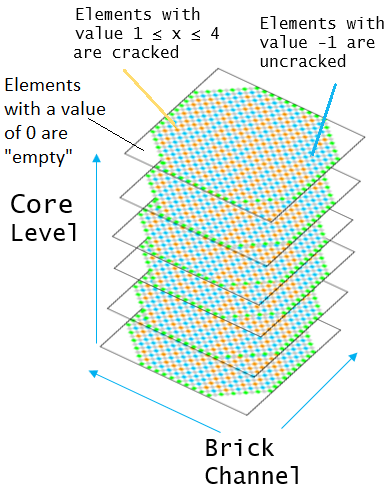
\includegraphics[scale=0.5]{Figures/cracked_core_array.png}
	\caption{AGR Input Core Tensor}
	\label{fig:core_array}
\end{figure}

\begin{figure}[ht!]
	\centering
	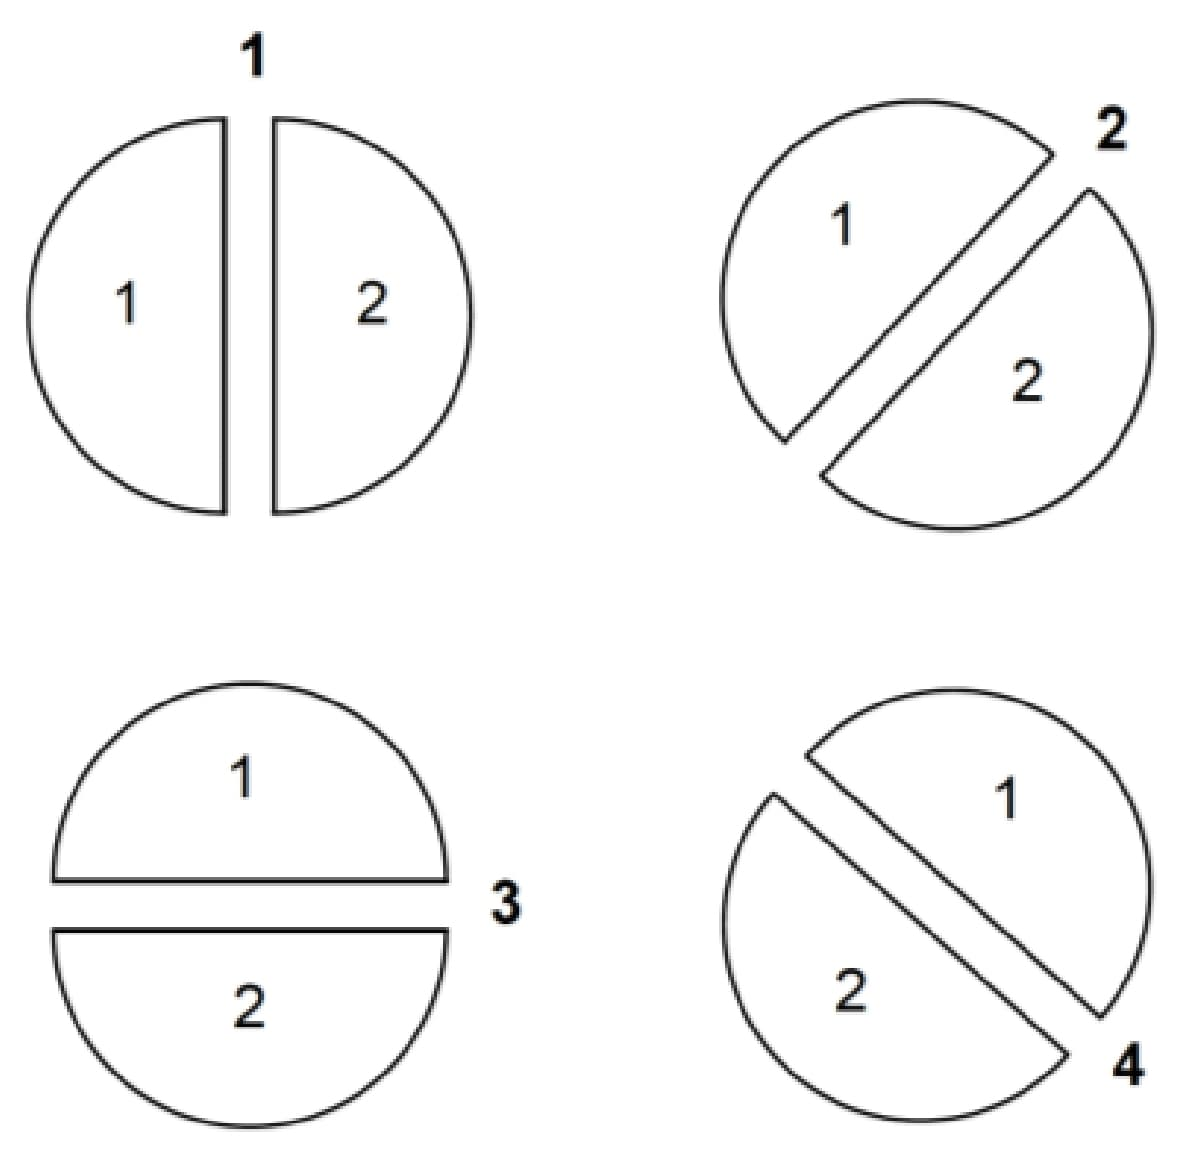
\includegraphics[scale=0.1]{Figures/orientations}
	\caption{Brick Crack Orientations}
	\label{fig:orientations}
\end{figure}

\noindent
An input tensor such as the example shown in Figure~\ref{fig:core_array} can be generated quickly and with low computational cost using industry standard tools (usually less than 1 minute per instance). These tensors can be used as input configurations to engineering models such as those shown in Figure~\ref{fig:FEA}~or~Figure~\ref{fig:ENG}. \\

\begin{figure}[ht!]
	\centering
	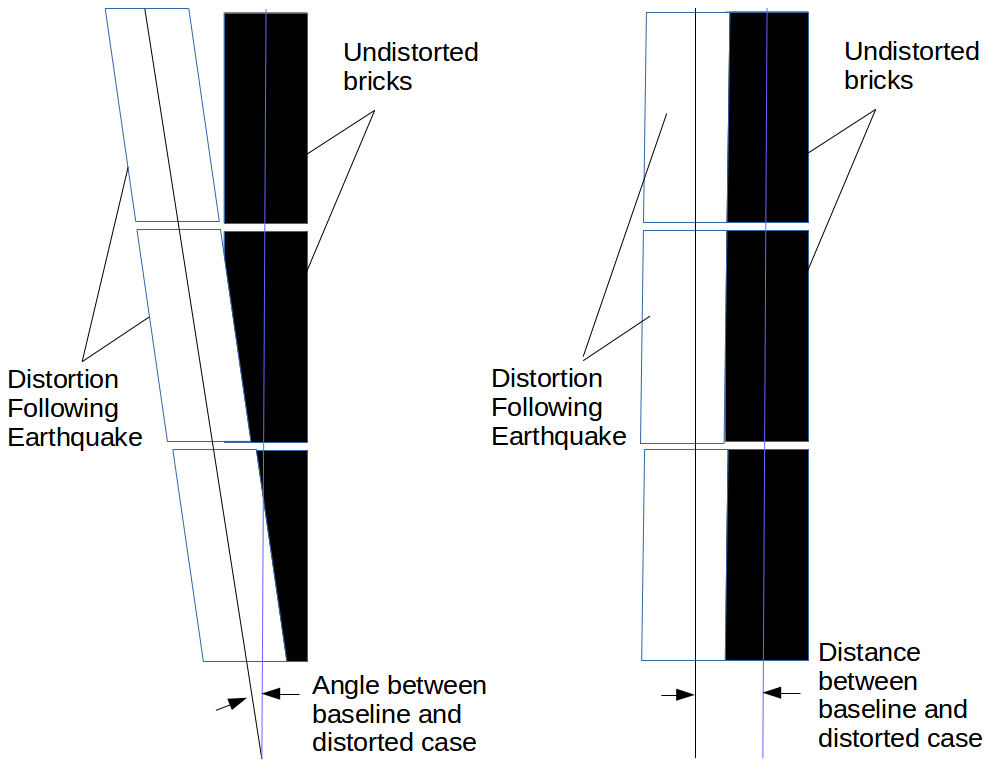
\includegraphics[scale=0.2]{Figures/Distored_bricks}
	\caption{Angle Between a Distorted and Baseline Brick Channel }
	\label{fig:angles}
\end{figure}

% 2D array
% Statistical Analysis

\noindent
The models are able to calculate the position of the bricks following an earthquake (Figure~\ref{fig:angles}) with the presence of cracked bricks influencing how the they move. Angular or translational movement of the bricks acts to effectively reduce the clearance between the fuel or control rod and the surrounding bore wall. Figure~\ref{fig:bore_clearance} illustrates an example involving an interstitial channel containing a control rod: the relative displacement of the control rod insertion point can be calculated as a function of the movement of the bricks. The path of the control rod must not be obstructed, and so the relative displacement must be less than the bore radius. \\

\begin{figure}[ht!]
	\centering
	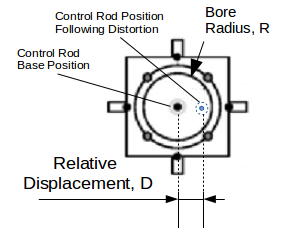
\includegraphics[scale=0.5]{Figures/bore_displacement}
	\caption{Relative Displacement of Control Rod}
	\label{fig:bore_clearance}
\end{figure}

\noindent
The outputs shown in Figures~\ref{fig:angles} \& \ref{fig:bore_clearance} are calculated for every interstitial brick of which there are 4173 in the Parmec model. Further complexity comes from the fact that the bricks move in and rotate around all three cardinal directions. There is also the time history of the earthquake to consider, with outputs generated at each time frame. 
\\

\noindent
A single iteration of the aforementioned process, summarised in Figure~\ref{fig:traditional}, gives us very little information on its own. With multiple iterations of this process, each with a different randomised state of the input tensor (Figure~\ref{fig:core_array}), a stochastic  understanding of the problem space can be built. For example, with several hundred iterations, a histogram can be plotted, as shown in Figure~\ref{fig:statistical_analysis}. The frequency of results is then fitted to a statistical distribution, such as the Normal distribution. Using this distribution, it can be determined what percentage of results are above an acceptable threshold (for instance, half the bore radius shown in \ref{fig:bore_clearance}). Using these statistics, determinations can be made of the probability of certain serious events occurring and are used in safety decision making.\\

\noindent
Both of the engineering modelling methods mentioned in this subsection are expensive in terms of time, computation and/or materials. This expense represents a significant bottleneck to the process summarised in Figure~\ref{fig:traditional}.\\


\begin{figure}[b!]
	\centering
	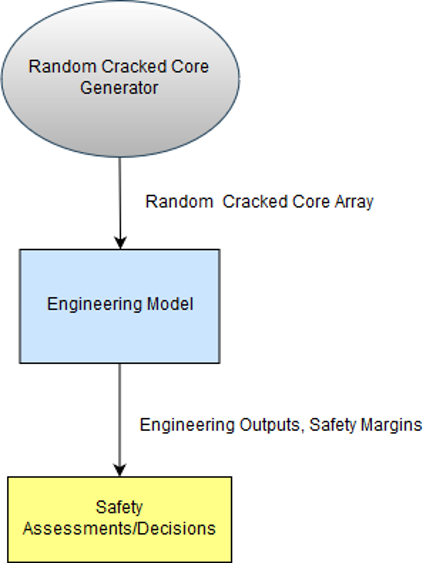
\includegraphics[scale=0.5]{Figures/engineering_approach}
	\caption{Traditional Engineering Approach}
	\label{fig:traditional}
\end{figure}

\begin{figure}[t]
	\centering
	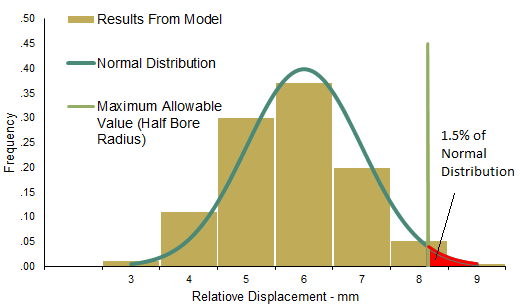
\includegraphics[scale=0.55]{Figures/Statistical_analysis}
	\caption{Statistical Analysis}
	\label{fig:statistical_analysis}
\end{figure}

\section{Parmec Model Description}

The computational model Parmec \cite{wiki:xxx} will serve as the traditional engineering model as the basis of this surrogate model to be developed for this PhD thesis. This section outlines the Parmec model, including how data is generated and the dimensionality of the inputs \& outputs. The full list of inputs and outputs to the Parmec model are summarised in Table~\ref{tab:parmecIO}.

\subsection{Data Generation} \label{parmec:data}

An individual Parmec case represents a simplified AGR graphite core with a cracked fuel bricks randomly distributed throughout. The Parmec software can simulate  a core with cracked bricks representing anywhere between 0\%  (intact core) and 100\% (fully cracked). Fuel bricks in the Parmec model can be modelled as having a single crack, or be double cracked as shown in Figure~\ref{fig:cracked}.  \\

\noindent
The configuration files for individual Parmec cases are generated using an industry standard tool which uses a pseudo-random number generated based on the time of day to distribute cracked bricks randomly throughout the core model. These configuration files contain the model inputs (discussed in the following subsection) and everything else required to execute Parmec. Following execution of the Parmec model using the configuration files, a set of output files are generated, the contents of which are discussed in subsection~\ref{parmec:output}. 

\subsection{Model Inputs} \label{parmec:input}

Fuel bricks are stacked in a multi-level structure as mentioned in section~\ref{AGR}. There are 7 levels (l~=~7), each with 284 bricks (f~=~284), hence there are 1988 fuel bricks in the reactor in total (r~=~1988). The input configuration files for a single Parmec case contain a integer representation of the cracking status of each brick in the core as visualised in Figure~\ref{fig:cascade}. In the aforementioned figure, an uncracked brick is represented by a -1, with cracked bricks represented by an integer 1 - 4, with this number giving the orientation (see Figure~\ref{fig:orientations}). Note that each core level has 18 rows and columns (d~=~18) but not every element represents a fuel brick - corner positions are padded with zeros.
\\

\begin{figure}[t]
	\centering
	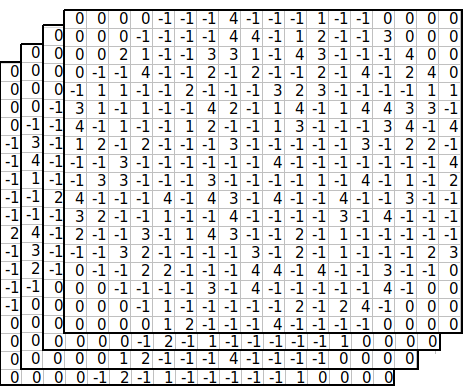
\includegraphics[scale=0.45]{Figures/InputCascade.png}
	\caption{Multi-channel Cascade}
	\label{fig:cascade}
\end{figure}

\subsection{Model Outputs} \label{parmec:output}

Recall from section~\ref{Engineering} that the Parmec model is used to simulate an earthquake (Figure~\ref{fig:earthquake}). This includes a settle down period before and after the earthquake proper. For 271 regular time intervals (TI) throughout the earthquake simulation, the model outputs a data-file. This file contains translation and rotation data for all bricks within the reactor core. 
\\

\noindent
There are 4173 interstitial bricks (henceforth referred to by the notation BI), the behaviour of which we are interested in during the earthquake time history. Like the fuel bricks discussed in the previous subsection, the interstitial bricks are stacked into channels. As the interstitials are shorter than their fuel equivalent, an interstitial channel is made of a stack of 13 bricks. Similar to the encoding process for fuel bricks, interstitials are encoded in order of their level and then by the order as given in Figure~\ref{fig:inter_order}.
\\

\noindent
For each interstitial brick, Parmec calculates 6 output metrics (OM) representing displacement in and rotation about all three Cartesian directions. With the 271 time intervals mentioned above, this results in nearly 6.8 million outputs per Parmec case. Therefore, each Parmec case has an output as can be represented by (\ref{instance_result_matrix}) with each value being normalised element-wise across the entire dataset.  
\\

\begin{figure}[t]
	\centering
	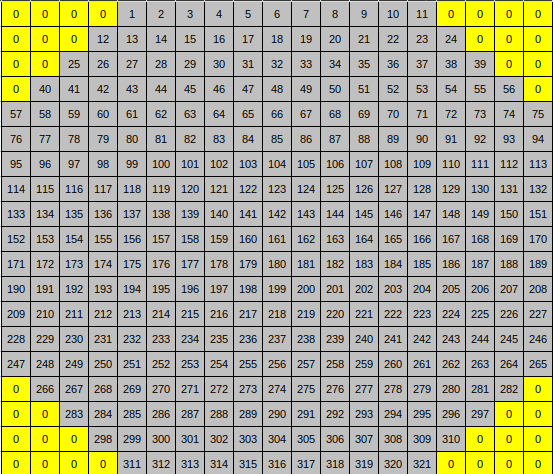
\includegraphics[scale=0.35]{Figures/inter_channel_numbers.png}
	\caption{Interstitial Brick Encoding Order}
	\label{fig:inter_order}
\end{figure}

\noindent


\begin{equation} \label{instance_result_matrix}
	Y_i = \{0, 1\}^{BI \ \times \ TI \ \times \ OM}
\end{equation}

\begin{table}[h!]
	\begin{center}
		
		\begin{tabular}{c|c|c|r|c} % <-- Alignments: 1st column left, 2nd middle and 3rd right, with vertical lines in between
			\textbf{Inputs} & \textbf{Outputs}  \\
			
			\hline
			& \\
			\textbf{Cracking Status}   &  \textbf{ Brick Displacement} \\
			1988 Fuel Bricks:         & 4173 Interstitial Bricks: \\ 
			7 levels    & 13 levels       \\
			284 fuel bricks per level &  321 bricks per level  \\
			&    \\
			& \textbf{Output Metrics}  \\
			& 6 per interstitial brick: \\ 
			
			&  3 translational \\
			&  3 rotational \\
			
			& \\
			
			\textbf{Earthquake Acceleration} & \textbf{Output Frequency} \\
			1400 time points: &              271 output points:     \\
			14 seconds &  once per 0.05 seconds    \\
			100 time points per second &     \\
			
			& \\
			
			Fuel brick cracking & Output for all \\
			status is constant & 4173 interstitial bricks \\
			throughout earthquake & and 6 output metrics \\
			& per time point \\
			
			
		\end{tabular}
		\caption{Summary of the Inputs and Outputs of the Parmec Engineering Model for AGR Graphite Core Seismic Analysis.}
		\label{tab:parmecIO}
	\end{center}
\end{table}


\begin{figure}[ht]
	\centering
	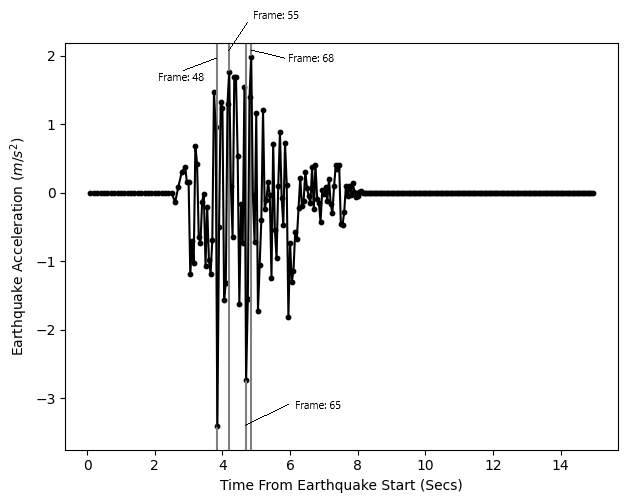
\includegraphics[scale=0.85]{Figures/earthquake_time_points}
	\caption{History of Acceleration During a Severe Earthquake} {Note the settling period before and after the earthquake proper. The true earthquake history includes an acceleration value every 100th of a second. This plot shows a sample every 10th of a second, which is the interval that the Parmec model outputs displacement data. Note that four time frames are highlighted - these frames are made reference to in the analysis in chapter~\ref{cha:dataset}.}
	\label{fig:earthquake}
\end{figure}




\section{Relevant Literature} \label{engineering:literature}

Calculations to ascertain the effects on the power plant following a severe earthquake were examined as early as the 1980s \cite{ahmed1986seismic} and 1990s \cite{allen1990seismic}. These works led to the more recent and detailed treatments of the problem, including \cite{kralj2007seismic} which uses a finite element analysis (FEA) model \cite{zienkiewicz2005finite} to simulate the behaviour of the core during an earthquake and generate a 3D output contour plot. \\

\noindent
The AGR reactor and its response to seismic activity is well studied in academic literature. In \cite{voyagaki2018earthquake}, both a computational and experimental examination of the AGR reactor is made. This paper discusses various seismic configurations, all involving an intact core i.e. without cracked bricks. The authors note that without cracking, an obstruction of a control rod channel during a seismic event is not possible due to the design of the core. \\

\noindent
A physical model representing the AGR core which includes randomly placed cracked bricks is described in \cite{dihoru2017development}. Elsewhere, \cite{oddbjornsson2017physical} looks at the effects of cracking in a physical AGR experiment at the University of Bristol. The results of these works help validate computational studies.\\ 

\noindent
These papers set the theoretical groundwork for this field, establish the methodology and make it clear that the response of the core is a function of input factors such as earthquake severity/direction. They also state some interesting results which may inform data/feature extraction, such as the most onerous results being near the upper and centre of the core.

